\documentclass[11pt,a4paper, twocolumn,
swedish, english %% Make sure to put the main language last!
]{article}
\pdfoutput=1

%% Andréas's custom package 
%% (Will work for most purposes, but is mainly focused on physics.)
\usepackage{custom_as}

%% Figures can now be put in a folder: 
\graphicspath{ {figures/} {figures/water/} {figures/good-fit/}
{figures/glycerol/} {figures/dual-diff/} {figures/example-waveform/}
}

%% If you want to change the margins for just the captions
\usepackage[size=small
]{caption}

%% To add todo-notes in the pdf
\usepackage[%disable  %%this will hide all notes
]{todonotes} 

%% Change the margin in the documents
\usepackage[
             top    = 3.0cm,              %% top margin
             bottom = 3.5cm,              %% bottom margin
             left   = 2.2cm, right  = 2.2cm %% left and right margins
]{geometry}


%% If you want to change the formatting of the section headers
%\renewcommand{\thesection}{...}

%\usepackage{abstract}
%\usepackage[affil-it]{authblk}
\usepackage{placeins}
%%%%%%%%%%%%%%%%%%%%%%%%%%%%%%%%%%%%%%%%%%%%%%%%%%%%%%%%%%%%%%%%%%%%%%
\begin{document}%% v v v v v v v v v v v v v v v v v v v v v v v v v v
%%%%%%%%%%%%%%%%%%%%%%%%%%%%%%%%%%%%%%%%%%%%%%%%%%%%%%%%%%%%%%%%%%%%%%

%%%%%%%%%%%%%%%%%%%% vvv Internal title page vvv %%%%%%%%%%%%%%%%%%%%%

\title{A qualitative investigation of self-diffusion in liquid water
  and glycerol and wet paper using the NMR pulse echo method} 
\author{Andréas Sundström$^*$%\footnote{\href{mailto:andsunds@student.chalmers.se}{andsunds@student.chalmers.se}}
  \and 
Tan Qin Yuan$^\dagger$%\footnote{\href{mailto:qiny@student.chalmers.se}{qiny@student.chalmers.se}}
}

\date{\today}

%\newgeometry{top    = 3.5cm,              %% top margin
%             bottom = 4cm,              %% bottom margin
%             left   = 3.5cm, right  = 3.5cm %% left and right margins
%}

\twocolumn[
\begin{@twocolumnfalse}
\vspace{-2cm}
\maketitle
\begin{abstract}
In this report the NMR pulse echo method is used to study
self-diffusion and the interaction between water and paper. A model,
by Carr~\&~Purcell, on the effects of diffusion on NMR pulse echoes is
presented and tested. Furthermore a dual water-layer theory, by
Perkins~\&~Batchelor, for the interaction between water and paper is
investigated. 
The samples tested were liquid water and glycerol; different degrees
of wet printer paper and wet tissue paper.
The results from the liquid water agree with the pulse echo diffusion
model. No diffusion could be observed in either glycerol or different
types of wet paper, this is ascribed to these samples having a too
high spin-spin relaxation rate, limiting the range of measurable
times. The dual water-layer theory is found to be able to explain
all our observations on (water) wet paper.
\end{abstract}

%This is such a bodgy solution to the problem. But hey! It works.
$^*${\footnotesize\href{mailto:andsunds@student.chalmers.se}{andsunds@student.chalmers.se}}
\\ %\hspace{50pt}
$^\dagger${\footnotesize\href{mailto:qiny@student.chalmers.se}{qiny@student.chalmers.se}}

\rule{\linewidth}{0.5pt}
\end{@twocolumnfalse}
]

%\clearpage
%\restoregeometry

%%%%%%%%%%%%%%%%%%%% ^^^ Internal title page ^^^ %%%%%%%%%%%%%%%%%%%%%
%% If you want a list of all todos
%\todolist



\section{Introduction}

As demands for increased rate of recycling and decreased use of fossil
products paper is a good alternative material for e.g. packaging
products, where the recycling rate of paper based packaging is as high
as 82\,\% in Sweden~\cite{Adolfson_NVV2016}. An increase in e-commerce
in the EU~\cite{eurostat_e-commerce2017} and other developed countries
also raises the demand for light-weight and durable cardboard
packaging~\cite{Nordstrand2003}. One major weakness of paper based 
packaging is however susceptibility to water damage which
significantly weakens the strength of the container; studies have even
shown the weakening effect of cyclic
humidity~\cite{Sorensen-Hoffmann2004} to paper products. It is 
therefore of great interest to study and understand the interaction
between water and paper products. 
One type of such paper-water interaction is the diffusion of water
into the paper and subsequent water self-diffusion inside the 
paper. This has been studied previously~\cite{Perkins-Batchelor2012,
  Li-etal1992, Topgaard-Soderman2001} for different water contents in
the paper. The diffusion of water in paper is not only important for
the end product, but it also plays a significant role in the
production and recycling of paper.

One of the main results by
Perkins~\&~Batchelor~\cite{Perkins-Batchelor2012} as well as by
Li~et~al.~\cite{Li-etal1992} was that water 
seemed to have two different modes of self-diffusion in paper, a fast
and a slow mode. Perkins~\&~Batchelor~\cite{Perkins-Batchelor2012}
further speculates that this is due to the water forming two different
layers around the cellulose fibers. All three of the diffusion
studies~\cite{Perkins-Batchelor2012, Li-etal1992,
  Topgaard-Soderman2001} have been using a technique called pulsed 
field gradient NMR. In this report we try to qualitatively replicate
some of the results by Perkins~\&~Batchelor using the
somewhat more primitive method of pulse echo NMR, developed by
Hahn~\cite{Hahn1950} and Carr~\&~Purcell~\cite{Carr-Purcell1954} in
the 1950's. We investigate the effects of self-diffusion in liquid
water and glycerol; we then compare the results to those of similar
measurements on wet printer paper and tissue paper with different
levels of moisture content. 



%Nuclear Magnetic Resonance refers to the phenomenon whereby nuclei of certain spin in the presence of an external magnetic field, undergo a transition of spin when exposed to a certain radio frequency. In the presence of a strong external magnetic field, the nuclei of the atoms of the sample undergo spin polarization. This is because any nuclei with magnetic moments that are not aligned with the direction of the magnetic field, experiences a magnetic torque which forces it to align to the direction of the magnetic field. The magnetic moment of the nuclei is perpendicular to the plane of spin of the nuclei. At the ground state (lower energy state), the magnetic moment of the nuclei is parallel to the direction of the magnetic field. However, when a certain radio frequency (Larmor frequency) is being transmitted onto the nuclei, some of the nuclei undergo Nuclear Magnetic Resonance. The nuclei on that ground state absorb photons of that frequency then transit to the excited energy state; refer to Fig 1. This happens by flipping the spin of the nuclei. The magnetic moments of the nuclei changes to anti-parallel to the direction of the magnetic field which corresponds to the excited state energy of the nuclei. If the resonance frequency (Larmor Frequency) source is turned off with the external magnetic field left on, the nuclei will then return to the ground state by reverting their spins and nuclear moments to parallel of the direction of the magnetic field. In the process, emitting photons of the Larmor Frequency. However, if both resonance frequency and external magnetic field are turned off, the nuclei will undergo random spontaneous emissions to return to its equilibrium state. At equilibrium state, the spin orientations and directions nuclear magnetic moments are random.   


\subsection{Pulsed NMR}

Nuclear Magnetic Resonance (NMR) refers to a method of probing the
spins of atomic nuclei, in an external magnetic field, by exciting
them with their resonance frequency, linked to the properties of the
nucleus and the external magnetic field. Some atomic nuclei have an
intrinsic spin, $\vb*I$, equivalent to the electron's. This energy of
the spin in an external magnetic field, $\vb*B_0$, is
\begin{equation}\label{eq:mag-energy}
E=-\gamma\vb*I\vdot\vb*B_0=-\gamma B_0 I_z
\end{equation}
(by convention $\vb*B_0=B_0\vu{z}$) similar to the Zeeman effect. Here
\begin{equation}
\gamma=\frac{ge}{2m_\text{p}},
\end{equation}
where $e$ is the charge of the proton, $m_\text{p}$ is the proton
mass, and $g$ is a dimensionless spectroscopic factor dependent on the
species of nucleus. This energy coupling, among all the nuclei in a
sample, will result in an aggregate macroscopic net magnetization,
$\vb*M$, parallel to $\vb*B_0$; it is this macroscopic magnetization which
can be probed in different ways using NMR techniques. 
While in principle NMR works for any types of nuclei with spin,
hydrogen ($^1\!$H) is the most used nucleus for NMR. This is because
$^1\!$H has one of the highest values of $\gamma$ among the common
chemical elements, certainly among the nuclei common to organic
chemistry. 

The principles of \emph{pulsed} NMR is that the equilibrium
magnetization can be disturbed using a pulsed, second magnetic field;
then the subsequent decay back to the equilibrium can be
measured. Any magnetic field, $\vb*B$, will exert a twisting torque on
$\vb*M$ according to
\begin{equation}
\vb*\tau=\vb*M\cross\vb*B.
\end{equation}
Since $\vb*\tau$ is perpendicular to both $\vb*M$ and $\vb*B$, the
torque results in a precession motion around $\vb*B$ with a
precession frequency \cite[ch. 2.1]{Principles_MR1990}
\begin{equation}
\omega_\text{L} = \gamma \abs{\vb*B}= \gamma B
\end{equation}
called the Larmor frequency. 
In the context of pulsed NMR there are two magnetic fields, the static
$\vb*B_0$ and the field from the pulse $\vb*B_1$ which is
perpendicular to $\vb*B_0$. Both will exert torques on $\vb*M$,
however since $B_0\gg B_1$ the precession around $\vb*B_0$ is
dominating. And unless $\vb*B_1$ stays in phase with the precession of
$\vb*M$ the time averaged effect of $\vb*B_1$ will diminish. That is
if $\vb*B_1$ rotates\footnotemark{} with angular frequency
$\omega_0=\gamma B_0$, then $\vb*B_1$ will have a lasting impact on
the magnetization $\vb*M$. That impact will be to rotate $\vb*M$
around $\vb*B_1$, away from $\vb*B_0$. It is here where the pulses
come into play; depending on the \emph{length} of the pulses, $\vb*M$
can be rotated by different amounts. Of special interest are the pulse
lengths which rotates $\vb*M$ by $90^\circ$ or $180^\circ$ -- called
$\pi/2$ and $\pi$ pulses respectively. Note that, in theory, the
$\pi/2$ pulse gives the strongest signal response while a $\pi$ pulse
should not give any signal at all.

\footnotetext{This would correspond to a circularly polarized
  field. In reality the fields used for $\vb*B_1$ are linearly
  polarized. However since any linearly polarized field can be
  split into two counter-rotating circularly polarized field this is
  no problem; one of the rotating component will keep in phase with the
  precession of $\vb*M$, while the other only generates very small
  perturbations. }

Now when the magnetization, $\vb*M$, has been rotated it will have a
component perpendicular to $\vb*B_0$. This perpendicular component,
$\vb*M_\perp$, rotates with angular frequency $\omega_0$. If a pick-up
coil is placed in this plane of rotation, $\vb*M_\perp$ will induce a
voltage which can be measured, and it is this measured voltage (or
rather its envelope) which is of interest in pulsed NMR
measurements. The signal will generally decay exponentially as
$\vb*M$ returns back to its equilibrium, the so called 
\emph{free induction decay}. The total exponential decay rate, by
convention called $R_2^*$ (sometimes also given as $T_2^*=1/R_2^*$),
can be said to generally consist of three terms 
\begin{equation}
R_2^*= R_1 + R_2 + \gamma\Delta B_0.
\end{equation}
The first two terms, $R_1$ and $R_2$, are related to the sample, and
the last term is from variations in $B_0$. These variations causes the
precession frequency to differ in different parts of the sample; the
spin precessions will therefore lose coherence and the signal will
decay. Unfortunately this last term often dominates. This means that
other methods must be used to measure $R_1$ and $R_2$ which are the
sample specific parameters. 

The first of the two intrinsic decay rates, $R_1$, the so called
\emph{longitudinal} or the \emph{spin-lattice} relaxation rate, is
related to the rate of energy loss of the spin. Since the
magnetization has been rotated the energy of the system has therefore
increased. The energy of the macroscopic magnetization is proportional
to $M_z$, similar to \eqref{eq:mag-energy}. The spin-lattice
relaxation rate is therefore related to the relaxation of $M_z$. We
will however not study or use this decay rate any further in this
report. 

%\subsubsection{The pulse echo method}
Instead we will focus on the second type of signal decay, $R_2$,
called the \emph{transverse} or the \emph{spin-spin} relaxation
rate. This decay rate is related to the coherentness of the individual
spins. As said before to measure any signal $M_\perp$ has to be
non-zero, which in turn requires the individual spins to be coherent
with each other. Consider an ideal ($\gamma\Delta B_0=0$) system
exposed by a $\pi/2$ pulse. Then directly after the pulse all the
spins have been rotated by $90^\circ$ in the same direction, which
means that $M_\perp$ is at its maximum. However If the spins, by some
intrinsic reason, tend to drift in phase when precessing, then
$M_\perp$ will decay due to loss of coherence -- similar to the signal
decay due to variations in $B_0$. It is that intrinsic individual
phase drift which gives rise to the decay of the signal corresponding
to $R_2$.  


\subsubsection{The pulse echo method and applying it to
measurements of the self-diffusion rate} 
\label{sec:pulse-echo}
In the previous example the static magnetic field, $B_0$, was assumed
to be completely homogeneous. However since the underlying mechanism
for signal decay due to $R_2$ and $\gamma\Delta B_0$ is the same, spin
de-coherence, it can be hard to separate these two decay modes. The
pulse echo method is a method for isolating  and measuring $R_2$. 

The key difference between the two modes of decay is that spin-spin
relaxation is due to intrinsic \emph{phase drift} due to fluctuations,
while the magnetic field variation leads to different precession
\emph{frequencies}. By the ingenious method of pulse echo by Erwin
Hahn~\cite{Hahn1950} in 1950. The most common type of pulse echo
measurements are done by applying a $\pi/2$ pulse followed by a number
of $\pi$ pulses.

To understand the effect of of the subsequent $\pi$ pulses assume that
$R_2=0$, i.e. that the only source of de-coherence is due to
variations in the precession frequency. The initial signal from the
$\pi/2$ pulse, at time $t=0$, will decay as usual then a $\pi$ pulse
at $t=\tau/2$ effectively flips all spins, including the
perpendicular components, $\vb*I_\perp\to-\vb*I_\perp$, of each
spin. The spins which had precessed faster due to having a slightly
higher precession frequency and was \emph{ahead} will now end up
\emph{behind}, but since they still have the faster frequency they
will catch up. At exactly time $t=\tau$ all the spins will meet
back up in phase, just like directly after the $\pi/2$ pulse, and an
identical signal would occur -- the ``pulse echo''. This can be
repeated with another $\pi$ pulse, usually at $t=3\tau/2$, to get
another echo. The echoes will only have the same amplitude if there
was no intrinsic rate of coherence loss. In reality the pulse echo
will decay in amplitude with rate $R_2$,
\begin{equation}
A(t)=A_0\exp[-R_2t].
\end{equation}

This is almost the whole picture. If the molecules in the sample can
diffuse to different regions with varying magnetic field,
Hahn~\cite{Hahn1950} showed that the signal will decay even faster if
diffusion is allowed. Afterwards
Carr~\&~Purcell~\cite{Carr-Purcell1954} further showed that the decay
is slowed when more pulses are used,
\begin{equation}\label{eq:echo-diffusion}
A(t)=A_0\exp(-R_2t)
\exp(-K\frac{t^3}{n^2}),
\end{equation}
where $n$ is the number of $\pi$ pulses before time $t$, and 
\begin{equation}\label{eq:K_simple}
K=\frac{\gamma^2D}{12}\qty(\pdv{B_0}{z})^2
\end{equation}
is a constant related to the diffusivity. Here $D$ is the
self-diffusivity of the sample, i.e. how fast a molecule of the sample
diffuses through it. There is also a strong dependence on the magnetic
field gradient $\pdv*{B_0}{z}$, which is linked to how fast the
precession frequency changes when a molecule diffuses.

Now if the $\pi$ pulses come at times
\begin{equation}\label{eq:pulse-times}
t_{n}=\qty(n-\tfrac{1}{2})\tau
\end{equation}
for some set pulse interval time $\tau$, then the echoes will occur at
time  
\begin{equation}
t_n'=n\tau.
\end{equation}
This means that \eqref{eq:echo-diffusion} can be written as
\begin{equation}\label{eq:multi-pulse_single}
A(t')=A_0\exp(-\mathcal{R}t')
\end{equation}
since the amplitude is only relevant at the time of the echoes, and
where 
\begin{equation}\label{eq:multi-pulse-rate}
\mathcal{R}=R_2+K\tau^2.
\end{equation}
By measuring the decay rate of the multi-pulse echoes, $\mathcal{R}$,
as a function of pulse interval, $\tau$, both the spin-spin relaxation
rate, $R_2$, and the self-diffusivity (indirectly), $D$, can be measured.

According to Perkins~\&~Batchelor~\cite{Perkins-Batchelor2012} water
has two modes of self-diffusion in paper with different diffusivities,
$D_1<D_2$; the first mode is called the slow mode and the second mode
is the fast for obvious reasons. Perkins~\&~Batchelor also mean that
this should manifest as a change of 
\eqref{eq:echo-diffusion} to
\begin{equation}
\begin{aligned}
A(t){=}\hspace{-1pt}A_0\hspace{1pt}
\ee^{{-}\!R_2t}\qty[
p\ee^{{-}K_1\!\frac{t^3}{n^2}} + (1{-}p)\ee^{{-}K_2\frac{t^3}{n^2}}
\!],
\end{aligned}
\end{equation}
with a similar modification to \eqref{eq:multi-pulse_single}
\begin{equation}\label{eq:multi-pulse_dual}
A(t')=A_0\qty[p\ee^{-\mathcal{R}_1t'}+
(1{-}p)\ee^{-\mathcal{R}_2t'}],
\end{equation}
where $K_1$, $K_2$, $\mathcal{R}_1$ and $\mathcal{R}_2$ (not to be
confused with $R_1$ and $R_2$) are defined analogously to
\eqref{eq:K_simple} and \eqref{eq:multi-pulse-rate}. The
scaling variable $0\le p\le1$ denotes the fraction of water in the
slow diffusion mode. 



\section{Method} \label{sec:met}
The main idea is to measure $A(t')$ for different values of $\tau$,
and then try to fit \eqref{eq:multi-pulse_single} to the measured
peaks of the pule echoes. From there we fit $R_2$ and $K$ to the
different observed decay rates $\mathcal{R}$ as a function of the
pulse interval, $\tau$, with \eqref{eq:multi-pulse-rate}. For the
measurements on wet paper we instead expect to find that
\eqref{eq:multi-pulse_dual} would give better results.

Different samples were placed in small test tubes, with an inner
diameter of about 5\,mm. These test tubes were then lowered into the
NMR apparatus consisting of two strong permanent magnets generating
$B_0$, radio frequency (RF) coils for generating $B_1$ and a pick-up
coil. The $B_1$ pulses were created with an accompanying pulse
programmer, RF oscillator and mixer, and RF receiver. The RF amplitude
envelope was then recorded on a digital oscilloscope, with which the
waveforms could be saved for later analysis. 
For doing the pulse echo measurements, three parameters need to be
calibrated -- the radio frequency, the length of the $\pi/2$ and $\pi$
pulses. These three parameters were re-calibrated before each
measurement to assure accurateness. The pulse programmer was such that
the $\pi$ pulses came as described in
\eqref{eq:pulse-times}. Furthermore the
Meiboom-Gill\cite{Meiboom-Gill1958} method for correcting slight
errors in the $\pi$ pulse length calibration was implemented -- these
types of pulses have no other effect on the theory described in
Section~\ref{sec:pulse-echo}. 

When the pulse echo measurements had been taken and saved, a script
was written to semi-automatically detect all the peaks
of the pulse echoes. Then the peaks were all fitted to either
\eqref{eq:multi-pulse_single} or \eqref{eq:multi-pulse_dual}.
Lastly the decay rates $\mathcal{R}$ (or $\mathcal{R}_{1, 2}$) was
plotted against $\tau^2$ to try and find a linear fit,
\eqref{eq:multi-pulse-rate}.\footnotemark{} 
This was primarily done for liquid water, as diffusion was fastest
there -- the diffusion in the other samples turned out to be too slow
to detect with this apparatus. 

\footnotetext{More detail on the data analysis can be found in
  Appendix~\ref{apx:data-analysis}. }

The samples tested were liquid water (distilled) and glycerol; 
printer paper and tissue paper. For brevity most investigation were
carried out on the printer paper, which will be referred to as just
``paper''. The printer paper samples were cut to a size of about  
$\unit[2]{cm}\times\unit[4]{cm}$ ($\unit[2]{cm}\times\unit[8]{cm}$ for
the tissue paper), wetted, folded lengthwise 2 times to about 5\,mm
width, and then the paper was rolled into a tight roll which fitted
snugly inside the test tubes.
The water wetted printer paper was examined for two different levels of
wetness, called either just ``wet'' or ``extra wet''; in the first
case the paper was thoroughly wetted with the liquid in question then
any excess liquid not soaked into the paper was wiped off with a dry
tissue, for ``extra wet'' paper an additional drop of liquid was added
to the sample when it was inside the test tube. We did not have the
equipment to do any quantitative water-to-paper ratio measurements,
which is why we only used these relatively crude terms of different
degrees of wetted paper.

As demonstrated by \eqref{eq:K_simple} this experiment is sensitive to
variations in $\pdv*{B_0}{z}$. We therefore took special care to make
each sample roughly the same size, as described in the previous
paragraph. Also the test tubes were marked so that each sample would 
be at the same location between the permanent magnets in the NMR
apparatus. To confirm the dependence of $\pdv*{B_0}{z}$ in
\eqref{eq:K_simple}, a measurement series for liquid water was also
taken with the sample moved off the mark by about 1\,mm, and then
compared to the same measurements on the mark. This also gave us a
sense of the sample positioning sensitivity of the experiment.



\section{Results}

\begin{figure}
\centering
% GNUPLOT: LaTeX picture with Postscript
\begingroup
  \makeatletter
  \providecommand\color[2][]{%
    \GenericError{(gnuplot) \space\space\space\@spaces}{%
      Package color not loaded in conjunction with
      terminal option `colourtext'%
    }{See the gnuplot documentation for explanation.%
    }{Either use 'blacktext' in gnuplot or load the package
      color.sty in LaTeX.}%
    \renewcommand\color[2][]{}%
  }%
  \providecommand\includegraphics[2][]{%
    \GenericError{(gnuplot) \space\space\space\@spaces}{%
      Package graphicx or graphics not loaded%
    }{See the gnuplot documentation for explanation.%
    }{The gnuplot epslatex terminal needs graphicx.sty or graphics.sty.}%
    \renewcommand\includegraphics[2][]{}%
  }%
  \providecommand\rotatebox[2]{#2}%
  \@ifundefined{ifGPcolor}{%
    \newif\ifGPcolor
    \GPcolortrue
  }{}%
  \@ifundefined{ifGPblacktext}{%
    \newif\ifGPblacktext
    \GPblacktexttrue
  }{}%
  % define a \g@addto@macro without @ in the name:
  \let\gplgaddtomacro\g@addto@macro
  % define empty templates for all commands taking text:
  \gdef\gplbacktext{}%
  \gdef\gplfronttext{}%
  \makeatother
  \ifGPblacktext
    % no textcolor at all
    \def\colorrgb#1{}%
    \def\colorgray#1{}%
  \else
    % gray or color?
    \ifGPcolor
      \def\colorrgb#1{\color[rgb]{#1}}%
      \def\colorgray#1{\color[gray]{#1}}%
      \expandafter\def\csname LTw\endcsname{\color{white}}%
      \expandafter\def\csname LTb\endcsname{\color{black}}%
      \expandafter\def\csname LTa\endcsname{\color{black}}%
      \expandafter\def\csname LT0\endcsname{\color[rgb]{1,0,0}}%
      \expandafter\def\csname LT1\endcsname{\color[rgb]{0,1,0}}%
      \expandafter\def\csname LT2\endcsname{\color[rgb]{0,0,1}}%
      \expandafter\def\csname LT3\endcsname{\color[rgb]{1,0,1}}%
      \expandafter\def\csname LT4\endcsname{\color[rgb]{0,1,1}}%
      \expandafter\def\csname LT5\endcsname{\color[rgb]{1,1,0}}%
      \expandafter\def\csname LT6\endcsname{\color[rgb]{0,0,0}}%
      \expandafter\def\csname LT7\endcsname{\color[rgb]{1,0.3,0}}%
      \expandafter\def\csname LT8\endcsname{\color[rgb]{0.5,0.5,0.5}}%
    \else
      % gray
      \def\colorrgb#1{\color{black}}%
      \def\colorgray#1{\color[gray]{#1}}%
      \expandafter\def\csname LTw\endcsname{\color{white}}%
      \expandafter\def\csname LTb\endcsname{\color{black}}%
      \expandafter\def\csname LTa\endcsname{\color{black}}%
      \expandafter\def\csname LT0\endcsname{\color{black}}%
      \expandafter\def\csname LT1\endcsname{\color{black}}%
      \expandafter\def\csname LT2\endcsname{\color{black}}%
      \expandafter\def\csname LT3\endcsname{\color{black}}%
      \expandafter\def\csname LT4\endcsname{\color{black}}%
      \expandafter\def\csname LT5\endcsname{\color{black}}%
      \expandafter\def\csname LT6\endcsname{\color{black}}%
      \expandafter\def\csname LT7\endcsname{\color{black}}%
      \expandafter\def\csname LT8\endcsname{\color{black}}%
    \fi
  \fi
    \setlength{\unitlength}{0.0500bp}%
    \ifx\gptboxheight\undefined%
      \newlength{\gptboxheight}%
      \newlength{\gptboxwidth}%
      \newsavebox{\gptboxtext}%
    \fi%
    \setlength{\fboxrule}{0.5pt}%
    \setlength{\fboxsep}{1pt}%
\begin{picture}(4534.00,4250.00)%
    \gplgaddtomacro\gplbacktext{%
      \csname LTb\endcsname%
      \put(620,640){\makebox(0,0)[r]{\strut{}0}}%
      \csname LTb\endcsname%
      \put(620,1314){\makebox(0,0)[r]{\strut{}2}}%
      \csname LTb\endcsname%
      \put(620,1988){\makebox(0,0)[r]{\strut{}4}}%
      \csname LTb\endcsname%
      \put(620,2661){\makebox(0,0)[r]{\strut{}6}}%
      \csname LTb\endcsname%
      \put(620,3335){\makebox(0,0)[r]{\strut{}8}}%
      \csname LTb\endcsname%
      \put(620,4009){\makebox(0,0)[r]{\strut{}10}}%
      \csname LTb\endcsname%
      \put(740,440){\makebox(0,0){\strut{}$0$}}%
      \csname LTb\endcsname%
      \put(1427,440){\makebox(0,0){\strut{}$500$}}%
      \csname LTb\endcsname%
      \put(2113,440){\makebox(0,0){\strut{}$1000$}}%
      \csname LTb\endcsname%
      \put(2800,440){\makebox(0,0){\strut{}$1500$}}%
      \csname LTb\endcsname%
      \put(3486,440){\makebox(0,0){\strut{}$2000$}}%
      \csname LTb\endcsname%
      \put(4173,440){\makebox(0,0){\strut{}$2500$}}%
    }%
    \gplgaddtomacro\gplfronttext{%
      \csname LTb\endcsname%
      \put(160,2324){\rotatebox{-270}{\makebox(0,0){\strut{}$\mathcal{R}$ /[$\unit{s^{-1}}$]}}}%
      \put(2456,140){\makebox(0,0){\strut{}$\tau^2$ /[$\unit{ms^2}$]}}%
      \csname LTb\endcsname%
      \put(3510,1053){\makebox(0,0)[r]{\strut{}\footnotesize On mark}}%
      \csname LTb\endcsname%
      \put(3510,853){\makebox(0,0)[r]{\strut{}\footnotesize Off mark}}%
    }%
    \gplbacktext
    \put(0,0){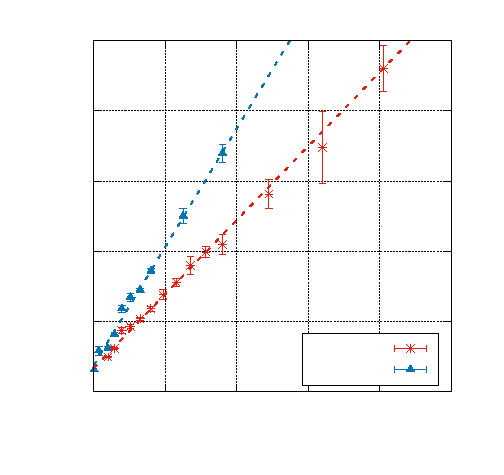
\includegraphics{water}}%
    \gplfronttext
  \end{picture}%
\endgroup

\caption{Amplitude decay rate $\mathcal{R}$ as a function of pulse
  interval squared $\tau^2$ for two different positions of a water
  sample. Linear fits to the two measurement series are also
  shown. Each data point is given with 95\,\% confidence interval. The
  ``off mark'' sample was moved to about 1\,mm off the mark which was
  used for the rest of the measurements in this report, which were
  ``on mark''. } 
\label{fig:water-pos}
\end{figure}

The first results of these measurements is the effect of sample
positioning inside the NMR apparatus. The result of the two
measurement series are shown in \figref{fig:water-pos}.
The parameters for the two linear fits, \eqref{eq:multi-pulse-rate},
were $R_2=\unit[0.67]{s^{-1}}$ and  
$K=\unit[4.21\times10^{-3}]{s^{-1}/ms^2}$ for the ``on mark'' water
measurements, and $R_2=\unit[0.76]{s^{-1}}$ and
$K=\unit[6.75\times10^{-3}]{s^{-1}/ms^2}$ for the ``off mark''.


\begin{figure}
\centering
% GNUPLOT: LaTeX picture with Postscript
\begingroup
  \makeatletter
  \providecommand\color[2][]{%
    \GenericError{(gnuplot) \space\space\space\@spaces}{%
      Package color not loaded in conjunction with
      terminal option `colourtext'%
    }{See the gnuplot documentation for explanation.%
    }{Either use 'blacktext' in gnuplot or load the package
      color.sty in LaTeX.}%
    \renewcommand\color[2][]{}%
  }%
  \providecommand\includegraphics[2][]{%
    \GenericError{(gnuplot) \space\space\space\@spaces}{%
      Package graphicx or graphics not loaded%
    }{See the gnuplot documentation for explanation.%
    }{The gnuplot epslatex terminal needs graphicx.sty or graphics.sty.}%
    \renewcommand\includegraphics[2][]{}%
  }%
  \providecommand\rotatebox[2]{#2}%
  \@ifundefined{ifGPcolor}{%
    \newif\ifGPcolor
    \GPcolortrue
  }{}%
  \@ifundefined{ifGPblacktext}{%
    \newif\ifGPblacktext
    \GPblacktexttrue
  }{}%
  % define a \g@addto@macro without @ in the name:
  \let\gplgaddtomacro\g@addto@macro
  % define empty templates for all commands taking text:
  \gdef\gplbacktext{}%
  \gdef\gplfronttext{}%
  \makeatother
  \ifGPblacktext
    % no textcolor at all
    \def\colorrgb#1{}%
    \def\colorgray#1{}%
  \else
    % gray or color?
    \ifGPcolor
      \def\colorrgb#1{\color[rgb]{#1}}%
      \def\colorgray#1{\color[gray]{#1}}%
      \expandafter\def\csname LTw\endcsname{\color{white}}%
      \expandafter\def\csname LTb\endcsname{\color{black}}%
      \expandafter\def\csname LTa\endcsname{\color{black}}%
      \expandafter\def\csname LT0\endcsname{\color[rgb]{1,0,0}}%
      \expandafter\def\csname LT1\endcsname{\color[rgb]{0,1,0}}%
      \expandafter\def\csname LT2\endcsname{\color[rgb]{0,0,1}}%
      \expandafter\def\csname LT3\endcsname{\color[rgb]{1,0,1}}%
      \expandafter\def\csname LT4\endcsname{\color[rgb]{0,1,1}}%
      \expandafter\def\csname LT5\endcsname{\color[rgb]{1,1,0}}%
      \expandafter\def\csname LT6\endcsname{\color[rgb]{0,0,0}}%
      \expandafter\def\csname LT7\endcsname{\color[rgb]{1,0.3,0}}%
      \expandafter\def\csname LT8\endcsname{\color[rgb]{0.5,0.5,0.5}}%
    \else
      % gray
      \def\colorrgb#1{\color{black}}%
      \def\colorgray#1{\color[gray]{#1}}%
      \expandafter\def\csname LTw\endcsname{\color{white}}%
      \expandafter\def\csname LTb\endcsname{\color{black}}%
      \expandafter\def\csname LTa\endcsname{\color{black}}%
      \expandafter\def\csname LT0\endcsname{\color{black}}%
      \expandafter\def\csname LT1\endcsname{\color{black}}%
      \expandafter\def\csname LT2\endcsname{\color{black}}%
      \expandafter\def\csname LT3\endcsname{\color{black}}%
      \expandafter\def\csname LT4\endcsname{\color{black}}%
      \expandafter\def\csname LT5\endcsname{\color{black}}%
      \expandafter\def\csname LT6\endcsname{\color{black}}%
      \expandafter\def\csname LT7\endcsname{\color{black}}%
      \expandafter\def\csname LT8\endcsname{\color{black}}%
    \fi
  \fi
    \setlength{\unitlength}{0.0500bp}%
    \ifx\gptboxheight\undefined%
      \newlength{\gptboxheight}%
      \newlength{\gptboxwidth}%
      \newsavebox{\gptboxtext}%
    \fi%
    \setlength{\fboxrule}{0.5pt}%
    \setlength{\fboxsep}{1pt}%
\begin{picture}(4534.00,4250.00)%
    \gplgaddtomacro\gplbacktext{%
      \csname LTb\endcsname%
      \put(620,640){\makebox(0,0)[r]{\strut{}30}}%
      \csname LTb\endcsname%
      \put(620,1202){\makebox(0,0)[r]{\strut{}35}}%
      \csname LTb\endcsname%
      \put(620,1763){\makebox(0,0)[r]{\strut{}40}}%
      \csname LTb\endcsname%
      \put(620,2325){\makebox(0,0)[r]{\strut{}45}}%
      \csname LTb\endcsname%
      \put(620,2886){\makebox(0,0)[r]{\strut{}50}}%
      \csname LTb\endcsname%
      \put(620,3448){\makebox(0,0)[r]{\strut{}55}}%
      \csname LTb\endcsname%
      \put(620,4009){\makebox(0,0)[r]{\strut{}60}}%
      \csname LTb\endcsname%
      \put(740,440){\makebox(0,0){\strut{}$0$}}%
      \csname LTb\endcsname%
      \put(1427,440){\makebox(0,0){\strut{}$10$}}%
      \csname LTb\endcsname%
      \put(2113,440){\makebox(0,0){\strut{}$20$}}%
      \csname LTb\endcsname%
      \put(2800,440){\makebox(0,0){\strut{}$30$}}%
      \csname LTb\endcsname%
      \put(3486,440){\makebox(0,0){\strut{}$40$}}%
      \csname LTb\endcsname%
      \put(4173,440){\makebox(0,0){\strut{}$50$}}%
    }%
    \gplgaddtomacro\gplfronttext{%
      \csname LTb\endcsname%
      \put(160,2324){\rotatebox{-270}{\makebox(0,0){\strut{}$\mathcal{R}$ /[$\unit{s^{-1}}$]}}}%
      \put(2456,140){\makebox(0,0){\strut{}$\tau^2$ /[$\unit{ms^2}$]}}%
      \csname LTb\endcsname%
      \put(2420,1253){\makebox(0,0)[r]{\strut{}\footnotesize Gylcerol paper}}%
      \csname LTb\endcsname%
      \put(2420,1053){\makebox(0,0)[r]{\strut{}\footnotesize Ex. glycerol paper}}%
      \csname LTb\endcsname%
      \put(2420,853){\makebox(0,0)[r]{\strut{}\footnotesize Liquid glycerol}}%
    }%
    \gplbacktext
    \put(0,0){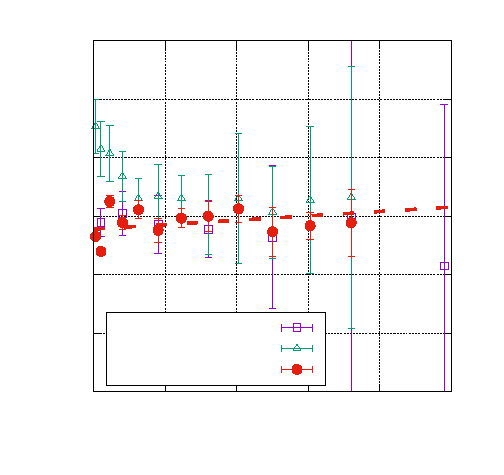
\includegraphics{glyc}}%
    \gplfronttext
  \end{picture}%
\endgroup

\caption{Amplitude decay rate $\mathcal{R}$ as a function of pulse
  interval squared $\tau^2$ for liquid glycerol, and printer paper
  wetted with glycerol. The error-bars signifies 95\,\% confidence
  intervals. The the two measurement series for wetted paper are for
  ``regularly'' wetted paper and ditto with one extra drop of glycerol
  added. }
\label{fig:glyc}
\end{figure}

Pulse echo measurement were performed for glycerol and
different levels of glycerol-wetted printer paper. The results are
shown in \figref{fig:glyc}. This time, the agreement with a linear fit
is much poorer, even for liquid glycerol, compared to the liquid water
in \figref{fig:water-pos}. Most measured values of $\mathcal{R}$ were
around $\mathcal{R}\approx\unit[45]{s^{-1}}$.


\begin{figure*}
\centering
% GNUPLOT: LaTeX picture with Postscript
\begingroup
  \makeatletter
  \providecommand\color[2][]{%
    \GenericError{(gnuplot) \space\space\space\@spaces}{%
      Package color not loaded in conjunction with
      terminal option `colourtext'%
    }{See the gnuplot documentation for explanation.%
    }{Either use 'blacktext' in gnuplot or load the package
      color.sty in LaTeX.}%
    \renewcommand\color[2][]{}%
  }%
  \providecommand\includegraphics[2][]{%
    \GenericError{(gnuplot) \space\space\space\@spaces}{%
      Package graphicx or graphics not loaded%
    }{See the gnuplot documentation for explanation.%
    }{The gnuplot epslatex terminal needs graphicx.sty or graphics.sty.}%
    \renewcommand\includegraphics[2][]{}%
  }%
  \providecommand\rotatebox[2]{#2}%
  \@ifundefined{ifGPcolor}{%
    \newif\ifGPcolor
    \GPcolortrue
  }{}%
  \@ifundefined{ifGPblacktext}{%
    \newif\ifGPblacktext
    \GPblacktexttrue
  }{}%
  % define a \g@addto@macro without @ in the name:
  \let\gplgaddtomacro\g@addto@macro
  % define empty templates for all commands taking text:
  \gdef\gplbacktext{}%
  \gdef\gplfronttext{}%
  \makeatother
  \ifGPblacktext
    % no textcolor at all
    \def\colorrgb#1{}%
    \def\colorgray#1{}%
  \else
    % gray or color?
    \ifGPcolor
      \def\colorrgb#1{\color[rgb]{#1}}%
      \def\colorgray#1{\color[gray]{#1}}%
      \expandafter\def\csname LTw\endcsname{\color{white}}%
      \expandafter\def\csname LTb\endcsname{\color{black}}%
      \expandafter\def\csname LTa\endcsname{\color{black}}%
      \expandafter\def\csname LT0\endcsname{\color[rgb]{1,0,0}}%
      \expandafter\def\csname LT1\endcsname{\color[rgb]{0,1,0}}%
      \expandafter\def\csname LT2\endcsname{\color[rgb]{0,0,1}}%
      \expandafter\def\csname LT3\endcsname{\color[rgb]{1,0,1}}%
      \expandafter\def\csname LT4\endcsname{\color[rgb]{0,1,1}}%
      \expandafter\def\csname LT5\endcsname{\color[rgb]{1,1,0}}%
      \expandafter\def\csname LT6\endcsname{\color[rgb]{0,0,0}}%
      \expandafter\def\csname LT7\endcsname{\color[rgb]{1,0.3,0}}%
      \expandafter\def\csname LT8\endcsname{\color[rgb]{0.5,0.5,0.5}}%
    \else
      % gray
      \def\colorrgb#1{\color{black}}%
      \def\colorgray#1{\color[gray]{#1}}%
      \expandafter\def\csname LTw\endcsname{\color{white}}%
      \expandafter\def\csname LTb\endcsname{\color{black}}%
      \expandafter\def\csname LTa\endcsname{\color{black}}%
      \expandafter\def\csname LT0\endcsname{\color{black}}%
      \expandafter\def\csname LT1\endcsname{\color{black}}%
      \expandafter\def\csname LT2\endcsname{\color{black}}%
      \expandafter\def\csname LT3\endcsname{\color{black}}%
      \expandafter\def\csname LT4\endcsname{\color{black}}%
      \expandafter\def\csname LT5\endcsname{\color{black}}%
      \expandafter\def\csname LT6\endcsname{\color{black}}%
      \expandafter\def\csname LT7\endcsname{\color{black}}%
      \expandafter\def\csname LT8\endcsname{\color{black}}%
    \fi
  \fi
    \setlength{\unitlength}{0.0500bp}%
    \ifx\gptboxheight\undefined%
      \newlength{\gptboxheight}%
      \newlength{\gptboxwidth}%
      \newsavebox{\gptboxtext}%
    \fi%
    \setlength{\fboxrule}{0.5pt}%
    \setlength{\fboxsep}{1pt}%
\begin{picture}(8502.00,4250.00)%
    \gplgaddtomacro\gplbacktext{%
      \csname LTb\endcsname%
      \put(860,640){\makebox(0,0)[r]{\strut{}$10^-4$}}%
      \csname LTb\endcsname%
      \put(860,1482){\makebox(0,0)[r]{\strut{}$10^-3$}}%
      \csname LTb\endcsname%
      \put(860,2325){\makebox(0,0)[r]{\strut{}$10^-2$}}%
      \csname LTb\endcsname%
      \put(860,3167){\makebox(0,0)[r]{\strut{}$10^-1$}}%
      \csname LTb\endcsname%
      \put(860,4009){\makebox(0,0)[r]{\strut{}$10^0$}}%
      \csname LTb\endcsname%
      \put(2852,440){\makebox(0,0){\strut{}$1$}}%
      \csname LTb\endcsname%
      \put(6433,440){\makebox(0,0){\strut{}$10$}}%
    }%
    \gplgaddtomacro\gplfronttext{%
      \csname LTb\endcsname%
      \put(160,2324){\rotatebox{-270}{\makebox(0,0){\strut{}$1-R^2$}}}%
      \put(4560,140){\makebox(0,0){\strut{}$\tau$ /[$\unit{ms}$]}}%
      \csname LTb\endcsname%
      \put(2468,3796){\makebox(0,0)[r]{\strut{}\footnotesize Liquid water}}%
      \csname LTb\endcsname%
      \put(2468,3596){\makebox(0,0)[r]{\strut{}\footnotesize Wet paper}}%
      \csname LTb\endcsname%
      \put(2468,3396){\makebox(0,0)[r]{\strut{}\footnotesize Ex. wet paper}}%
    }%
    \gplbacktext
    \put(0,0){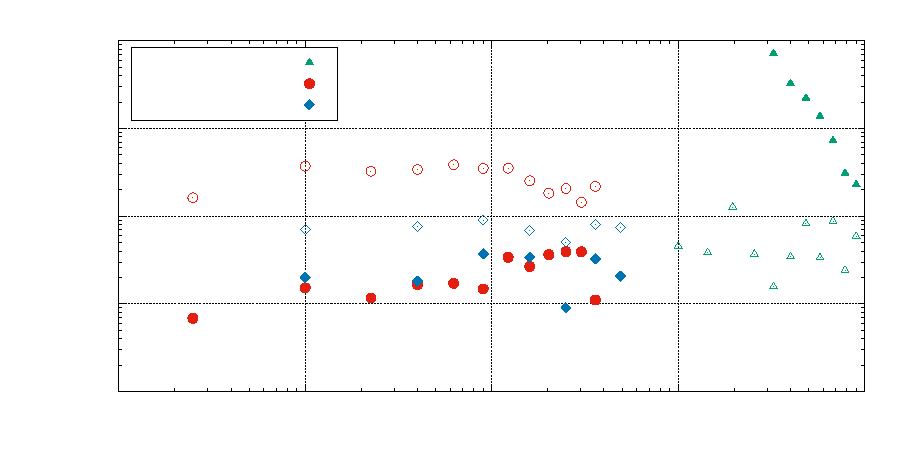
\includegraphics{fit_Rsq}}%
    \gplfronttext
  \end{picture}%
\endgroup

\caption{One minus confidence of determination ($1-r^2$),
  fit degree-of-freedom adjusted, for the fits using either the single
  mode diffusion model (open markers) or dual mode diffusion (solid
  markers) for different samples. [Lower values means better fits.]
  The horizontal axis is the pulse interval, $\tau$, but has no
  significance to the $r^2$ values. Examples of the goodness of the
  differnt fits are shown in \figref{fig:fitted-peaks} in
  Appendix~\ref{apx:data-analysis}. 
} 
\label{fig:good-fit}
\end{figure*}

To examine whether the dual diffusion mode theory better corresponds
to the measurements, \figref{fig:good-fit} presents the
degree-of-freedom adjusted confidence of determination (colloquially
known as ``R-squared'') for fits to the data either by
\eqref{eq:multi-pulse_single} or \eqref{eq:multi-pulse_dual}. The
figure shows one minus the R-squared values for liquid water, extra
wet printer paper, and wet tissue paper. Corresponding values for other
samples are omitted form the figure, partly to not make it too
crowded, and partly because they did not show any separation between
the two theories. There is a clear separation between the two theories for
both liquid water and extra wet printer paper -- the wet tissue paper
also shows some separation but it is less
pronounced. Do note however that the separations are in opposite
directions; the single mode theory fits better to the liquid water
than dual mode diffusion, while the opposite is true for extra wet
paper -- and to some extent wet tissue paper. Examples of the
fits of the two decay modes are shown in \figref{fig:fitted-peaks} in
Appendix~\ref{apx:data-analysis}. 


\begin{figure*}
\centering
% GNUPLOT: LaTeX picture with Postscript
\begingroup
  \makeatletter
  \providecommand\color[2][]{%
    \GenericError{(gnuplot) \space\space\space\@spaces}{%
      Package color not loaded in conjunction with
      terminal option `colourtext'%
    }{See the gnuplot documentation for explanation.%
    }{Either use 'blacktext' in gnuplot or load the package
      color.sty in LaTeX.}%
    \renewcommand\color[2][]{}%
  }%
  \providecommand\includegraphics[2][]{%
    \GenericError{(gnuplot) \space\space\space\@spaces}{%
      Package graphicx or graphics not loaded%
    }{See the gnuplot documentation for explanation.%
    }{The gnuplot epslatex terminal needs graphicx.sty or graphics.sty.}%
    \renewcommand\includegraphics[2][]{}%
  }%
  \providecommand\rotatebox[2]{#2}%
  \@ifundefined{ifGPcolor}{%
    \newif\ifGPcolor
    \GPcolortrue
  }{}%
  \@ifundefined{ifGPblacktext}{%
    \newif\ifGPblacktext
    \GPblacktexttrue
  }{}%
  % define a \g@addto@macro without @ in the name:
  \let\gplgaddtomacro\g@addto@macro
  % define empty templates for all commands taking text:
  \gdef\gplbacktext{}%
  \gdef\gplfronttext{}%
  \makeatother
  \ifGPblacktext
    % no textcolor at all
    \def\colorrgb#1{}%
    \def\colorgray#1{}%
  \else
    % gray or color?
    \ifGPcolor
      \def\colorrgb#1{\color[rgb]{#1}}%
      \def\colorgray#1{\color[gray]{#1}}%
      \expandafter\def\csname LTw\endcsname{\color{white}}%
      \expandafter\def\csname LTb\endcsname{\color{black}}%
      \expandafter\def\csname LTa\endcsname{\color{black}}%
      \expandafter\def\csname LT0\endcsname{\color[rgb]{1,0,0}}%
      \expandafter\def\csname LT1\endcsname{\color[rgb]{0,1,0}}%
      \expandafter\def\csname LT2\endcsname{\color[rgb]{0,0,1}}%
      \expandafter\def\csname LT3\endcsname{\color[rgb]{1,0,1}}%
      \expandafter\def\csname LT4\endcsname{\color[rgb]{0,1,1}}%
      \expandafter\def\csname LT5\endcsname{\color[rgb]{1,1,0}}%
      \expandafter\def\csname LT6\endcsname{\color[rgb]{0,0,0}}%
      \expandafter\def\csname LT7\endcsname{\color[rgb]{1,0.3,0}}%
      \expandafter\def\csname LT8\endcsname{\color[rgb]{0.5,0.5,0.5}}%
    \else
      % gray
      \def\colorrgb#1{\color{black}}%
      \def\colorgray#1{\color[gray]{#1}}%
      \expandafter\def\csname LTw\endcsname{\color{white}}%
      \expandafter\def\csname LTb\endcsname{\color{black}}%
      \expandafter\def\csname LTa\endcsname{\color{black}}%
      \expandafter\def\csname LT0\endcsname{\color{black}}%
      \expandafter\def\csname LT1\endcsname{\color{black}}%
      \expandafter\def\csname LT2\endcsname{\color{black}}%
      \expandafter\def\csname LT3\endcsname{\color{black}}%
      \expandafter\def\csname LT4\endcsname{\color{black}}%
      \expandafter\def\csname LT5\endcsname{\color{black}}%
      \expandafter\def\csname LT6\endcsname{\color{black}}%
      \expandafter\def\csname LT7\endcsname{\color{black}}%
      \expandafter\def\csname LT8\endcsname{\color{black}}%
    \fi
  \fi
    \setlength{\unitlength}{0.0500bp}%
    \ifx\gptboxheight\undefined%
      \newlength{\gptboxheight}%
      \newlength{\gptboxwidth}%
      \newsavebox{\gptboxtext}%
    \fi%
    \setlength{\fboxrule}{0.5pt}%
    \setlength{\fboxsep}{1pt}%
\begin{picture}(8502.00,5102.00)%
    \gplgaddtomacro\gplbacktext{%
      \csname LTb\endcsname%
      \put(620,640){\makebox(0,0)[r]{\strut{}0}}%
      \csname LTb\endcsname%
      \put(620,1344){\makebox(0,0)[r]{\strut{}10}}%
      \csname LTb\endcsname%
      \put(620,2047){\makebox(0,0)[r]{\strut{}20}}%
      \csname LTb\endcsname%
      \put(620,2751){\makebox(0,0)[r]{\strut{}30}}%
      \csname LTb\endcsname%
      \put(620,3454){\makebox(0,0)[r]{\strut{}40}}%
      \csname LTb\endcsname%
      \put(620,4158){\makebox(0,0)[r]{\strut{}50}}%
      \csname LTb\endcsname%
      \put(620,4861){\makebox(0,0)[r]{\strut{}60}}%
      \csname LTb\endcsname%
      \put(740,440){\makebox(0,0){\strut{}$0$}}%
      \csname LTb\endcsname%
      \put(2220,440){\makebox(0,0){\strut{}$10$}}%
      \csname LTb\endcsname%
      \put(3700,440){\makebox(0,0){\strut{}$20$}}%
      \csname LTb\endcsname%
      \put(5181,440){\makebox(0,0){\strut{}$30$}}%
      \csname LTb\endcsname%
      \put(6661,440){\makebox(0,0){\strut{}$40$}}%
      \csname LTb\endcsname%
      \put(8141,440){\makebox(0,0){\strut{}$50$}}%
    }%
    \gplgaddtomacro\gplfronttext{%
      \csname LTb\endcsname%
      \put(160,2750){\rotatebox{-270}{\makebox(0,0){\strut{}$\mathcal{R}$ /[$\unit{s^{-1}}$]}}}%
      \put(4440,140){\makebox(0,0){\strut{}$\tau^2$ /[$\unit{ms^2}$]}}%
      \csname LTb\endcsname%
      \put(7478,4648){\makebox(0,0)[r]{\strut{}\footnotesize Ex. wet printer paper}}%
      \csname LTb\endcsname%
      \put(7478,4448){\makebox(0,0)[r]{\strut{}\footnotesize Wet tissue paper}}%
    }%
    \gplbacktext
    \put(0,0){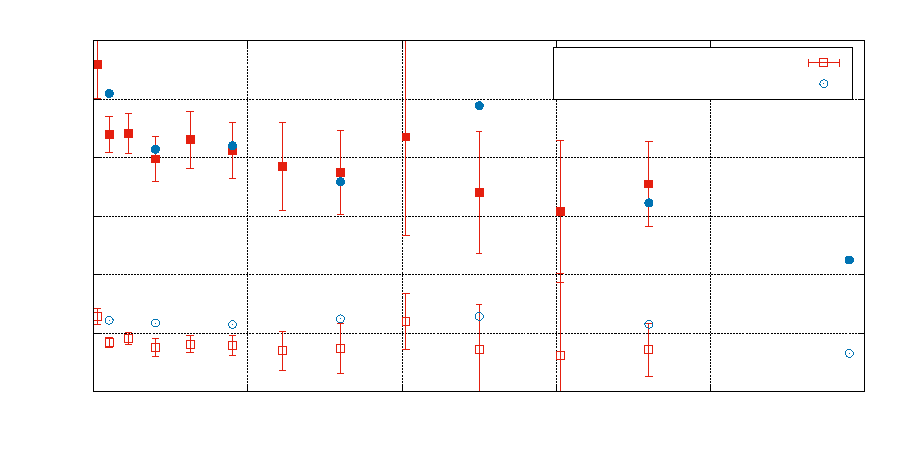
\includegraphics{diff}}%
    \gplfronttext
  \end{picture}%
\endgroup

\caption{Amplitude decay rate $\mathcal{R}$ as a function of pulse
  interval squared $\tau^2$ for the fast (solid markers) and slow
  (open markers) decay mode of water in extra wet printer paper or
  tissue paper. The data points for extra wet printer paper is given
  with 95\,\% confidence intervals. (The error-bars for the tissue
  paper is omitted for clarity in the plot.) } 
\label{fig:dual-diff}
\end{figure*}

The dual decay mode theory, \eqref{eq:multi-pulse_dual}, was fitted to
the measured pulse echo amplitudes for extra wet printer paper and
tissue paper. These samples were chosen 
The two decay rates for the two samples are presented in
\figref{fig:dual-diff}. There is a somewhat clear resemblance between
the two samples in terms of separation between the slow and the fast
mode of decay. Also note the much higher decay rates compared to pure
liquid  water, even for the slow modes. The values of $p$
(corresponding to the fraction of water in the slow mode) were all
quite sable except for a few outliers for each sample. However, the
two samples had significantly different $p$ values. The extra wet
printer paper had values around $p=0.25\pm0.05$, while the tissue
paper had values of $p=0.7\pm0.1$.

For the ``regular'' wet paper, the R-squared values showed no
particular preference either way between the two suggested modes of
decay. The single mode decay rates for wet paper were, for all
measured $\tau$ between 0.5\,ms and 6.0\,ms, around
$\mathcal{R}\approx\unit[50]{s^{-1}}$. 


\section{Discussion}

We can primarily draw two conclusions from \figref{fig:water-pos}. The
first one is that the static magnetic field, $B_0$, is too non-uniform
in our apparatus to be able to do any quantitative diffusivity
calculations. This is due to the large difference in slopes from just
a small change, of around 1\,mm, in sample position. The parameter
$K$, from which the diffusivity would be derived, changed by 60\,\%
for the ``off mark'' sample compared to the ``on mark''. Furthermore,
the rest of the measurements are supposed to be on the mark, however
that was hard to gauge when inserting the samples into the NMR
devise. We estimate that the position uncertainty probably lies in the
range of at least $\pm\unit[0.5]{mm}$, which promptly makes any
quantitative diffusivity measurements unusably uncertain.

The second main conclusion from \figref{fig:water-pos} is that our
data suggests that the diffusion effect, \eqref{eq:echo-diffusion} by
Carr~\&~Purcell~\cite{Carr-Purcell1954}, is valid. By the same
argument as in the previous paragraph, we can however not draw any
conclusions regarding the validity of the quantitative expression in
\eqref{eq:K_simple}. The conclusion we can draw is that the
qualitative relation \eqref{eq:multi-pulse-rate} between the pulse
interval, $\tau$, and the observed pulse echo amplitude decay rate,
$\mathcal{R}$. This relationship was directly derived from
\eqref{eq:echo-diffusion}, which therefore also suggests the
qualitative validity of ditto. That is, our measurements suggests that
there is a second exponential decay, and that the second exponential
decay has a $t^3/n^2$ time and pulse number dependence. 

Although any conclusions regarding diffusivity are only
qualitative, we can however obtain one quantitative result from
\figref{fig:water-pos}. That is the intrinsic spin-spin relaxation
rate $R_2$. The two measurement series both converge at around
$R_2\approx\unit[0.7]{s^{-1}}$ ($T_2=1/R_2\approx\unit[1.4]{s}$) when
$\tau\to0$. This is further testimony 
of the validity of \eqref{eq:multi-pulse-rate} and
\eqref{eq:echo-diffusion}. Other studies have gotten results of
$R_2=\unit[0.39]{s^{-1}}$~\cite{Sabadini-etal2008}
($T_2=\unit[2.56]{s}$), which is almost half of what we
found. However different impurities can strongly affect the values of
$R_2$, as shown by both~\cite{Sabadini-etal2008}
and~\cite{Nelson-etal2002}. For instance,~\cite{Sabadini-etal2008}
showed that $R_2$ gets as high as $\unit[1.70]{s^{-1}}$ with only
1\,\% glucose in the solution. We used distilled water and tried to
rinse out all the test tubes before use to try and mitigate any
impurities. However we believe that we did have some impurities in
the end which would explain our rather high value of $R_2$ for ``pure
water''.  

As for the glycerol in \figref{fig:glyc}, very little can be said
about the diffusion unfortunately. The measurements were taken with a
too narrow range of pulse intervals, $\tau$, to be able to say 
anything on whether or not there even is a linear relationship
between $\mathcal{R}$ and $\tau^2$ in \figref{fig:glyc}. Note, for
instance, that the clear linear patterns in \figref{fig:water-pos} are
over a range of $\tau^2$ that is 50~times greater; a line with the
same slope as in \figref{fig:water-pos} would look almost completely
flat in \figref{fig:glyc}. The reason why we were restricted to this
narrow range of pulse intervals is due to the fast intrinsic decay rate
observed $R_2\approx\mathcal{R}\approx\unit[45]{s^{-1}}$, lying two
orders of magnitude above that of water. This meant that the signal
would have decayed down to undetectable levels for any longer pulse
intervals, hence the short range of $\tau$.

Unfortunately much the same is true for measurements in
\figref{fig:dual-diff}. The range of $\tau^2$ is much too short to say
anything about any difference in diffusion rates between the fast and
slow decay-mode, i.e. slopes in the graph, which was the goal of this
report. Ideally we would have observed a pattern similar to that of
\figref{fig:water-pos}, but instead of two different sample positions
the two lines would have arose from a fast and slow mode of
diffusion. This is not what we see. \figref{fig:dual-diff} shows two
quite clearly separated modes of signal decay, running almost parallel
along the whole range of $\tau^2$.

However \figref{fig:good-fit}, together with the example in
\figref{fig:fitted-peaks} in Appendix~\ref{apx:data-analysis},
strongly suggest that the deay of extra wet printer paper and tissue
paper follows a dual decay rate model rather than single decay rate.
This could be due to the increased number of fit parameters
which makes it easier to fit a function to data. The values presented
in \figref{fig:good-fit} are however the so called
``degree-of-freedom adjusted'' R-squared values as calculated by
Matlab's \texttt{fit} function, see \cite{Matlab-fit}. We do not know the
full details, but it is reasonable to believe that this means that the
better fits of the dual decay rate model actually stems from better
agreement with reality rather than just it having more fit
parameters. Also the example in \figref{fig:fitted-peaks} clearly
shows that a single decay rate does not represent the data very well
at all.

It is furthermore conceivable that we should expect two different
spin-spin decay rates, $R_2$, in wet paper -- as observed in
\figref{fig:dual-diff}. Perkins~\&~Batchelor~\cite{Perkins-Batchelor2012}
speculates that their observed dual modes of diffusion can be due to
the water splitting up in two layers, one inner layer close to the
cellulose fibers and one outer layer which consists of more free water
molecules. 
The two different diffusion modes are then attributed to these two
water-layers~\cite{Perkins-Batchelor2012}. Although
Perkins~\&~Batchelor themselves do not present any values of $R_2$ for
the two different layers, we do however know that water interacting
with cellulose increases the value of $R_2$~\cite{Ono-etal2004}.

If this water-layer theory is true, then we would expect that the
inner water-layer would have stronger interaction with the cellulose
and therefore have a higher $R_2$. We also note that the ``regular wet
paper'' did not show any appreciable difference between single and
dual mode decays, however the (single mode) decay rates in the regular
wet paper are similar to those of the fast decay modes in
\figref{fig:dual-diff}. This could be explained by the regular wet
paper not having enough water to form an outer layer with the slower
decay rates, and instead only forming an inner water-layer.
This would also explain why the regular wet paper showed the same
decay rate as the ``fast'' rate in \figref{fig:dual-diff}.

One possible fact that might speak against the dual water-layer
theory is the fact that the value of $p$ differed so distinctly
between the extra wet printer paper and the tissue paper. However the
printer paper is much more dense then the tissue paper, which would
mean that the water-to-paper ratio might have been much higher in the
tissue paper than in the extra wet printer paper. We would therefore
expect $p$, which corresponds to the fraction of water in the slow
decay mode, to be higher for tissue paper due to the higher water
content accumulating in the outer layer. And indeed that is what we
observed. 

For the glycerol-wetted paper in \figref{fig:glyc}, there is however
not an appreciable change in $R_2$ or any indication of dual
decay rates. This might be due to glycerol having a much weaker
interaction with cellulose. Glycerol, being a larger molecule, might
also not form a thin inner layer around the fibers, as is suggested
that water does. 




%\todo[inline]{Funky bussiness happening for low $\tau$ in
%  \figref{fig:dual-diff}. }



\section{Conclusions}

%In conclusion, we only considered quantitative results due to the due to unreliability of results of diffusitivity. Experiments were done for "extra wet","wet" and dry paper. No results were seen in dry paper due to its molecular structure. Not much difference can be inferred from "extra wet" and "wet" paper, possibly due to limitations of equipment and experimental method. 

For liquid samples with slow intrinsic spin-spin decay rates $R_2$,
where diffusion could present a problem to measurements of $R_2$, the
Carr~\&~Purcell method can be used to extract the value of
$R_2$, using \eqref{eq:multi-pulse-rate}. This is only necessary for
samples where $R_2$ is quite small ($R_2\sim K\tau^2$), like
water. The effects of diffusion are however negligible in time scales
of around $T_2=1/R_2$, which would be the case for samples with higher
$R_2$ and/or slower diffusion ($R_2\gg K\tau^2$), like glycerol. 

We could not measure any diffusion in wet paper, no less two distinct
modes of diffusion. Our data do however suggest that the wet paper
has two distinct values of $R_2$. This can be explained by the dual
water-layer theory by Perkins~\&~Batchelor. This dual water-layer
theory is also supported by the fact that the measured $R_2$ values
of paper with lower water content agrees with that of the fast decay
mode in extra wet paper. 



%\section{References}
%http://hyperphysics.phy-astr.gsu.edu/hbase/Nuclear/nmr.html

%%%%%%%%%%%%%%%%%%%%%%%%%% The bibliography %%%%%%%%%%%%%%%%%%%%%%%%%%
\clearpage
%% This bibliography uses BibTeX
\bibliographystyle{ieeetr}
\bibliography{references}%requires a file named 'references.bib'
%% Citations are as usual: \cite{example_article}

%%%%%%%%%%%%%%%%%%%%%%%%%%%%% Appendices %%%%%%%%%%%%%%%%%%%%%%%%%%%%%
\clearpage %% on a new page 
\appendix  %% This will change the page numbering to A1, A2, A3, ...;
           %% and also change the sections to A, A.1, ...; B, B.1, ...

\section{Detailed data analysis 
with examples of the observed raw-data}
\label{apx:data-analysis}

\begin{figure*}
\centering
% GNUPLOT: LaTeX picture with Postscript
\begingroup
  \makeatletter
  \providecommand\color[2][]{%
    \GenericError{(gnuplot) \space\space\space\@spaces}{%
      Package color not loaded in conjunction with
      terminal option `colourtext'%
    }{See the gnuplot documentation for explanation.%
    }{Either use 'blacktext' in gnuplot or load the package
      color.sty in LaTeX.}%
    \renewcommand\color[2][]{}%
  }%
  \providecommand\includegraphics[2][]{%
    \GenericError{(gnuplot) \space\space\space\@spaces}{%
      Package graphicx or graphics not loaded%
    }{See the gnuplot documentation for explanation.%
    }{The gnuplot epslatex terminal needs graphicx.sty or graphics.sty.}%
    \renewcommand\includegraphics[2][]{}%
  }%
  \providecommand\rotatebox[2]{#2}%
  \@ifundefined{ifGPcolor}{%
    \newif\ifGPcolor
    \GPcolortrue
  }{}%
  \@ifundefined{ifGPblacktext}{%
    \newif\ifGPblacktext
    \GPblacktexttrue
  }{}%
  % define a \g@addto@macro without @ in the name:
  \let\gplgaddtomacro\g@addto@macro
  % define empty templates for all commands taking text:
  \gdef\gplbacktext{}%
  \gdef\gplfronttext{}%
  \makeatother
  \ifGPblacktext
    % no textcolor at all
    \def\colorrgb#1{}%
    \def\colorgray#1{}%
  \else
    % gray or color?
    \ifGPcolor
      \def\colorrgb#1{\color[rgb]{#1}}%
      \def\colorgray#1{\color[gray]{#1}}%
      \expandafter\def\csname LTw\endcsname{\color{white}}%
      \expandafter\def\csname LTb\endcsname{\color{black}}%
      \expandafter\def\csname LTa\endcsname{\color{black}}%
      \expandafter\def\csname LT0\endcsname{\color[rgb]{1,0,0}}%
      \expandafter\def\csname LT1\endcsname{\color[rgb]{0,1,0}}%
      \expandafter\def\csname LT2\endcsname{\color[rgb]{0,0,1}}%
      \expandafter\def\csname LT3\endcsname{\color[rgb]{1,0,1}}%
      \expandafter\def\csname LT4\endcsname{\color[rgb]{0,1,1}}%
      \expandafter\def\csname LT5\endcsname{\color[rgb]{1,1,0}}%
      \expandafter\def\csname LT6\endcsname{\color[rgb]{0,0,0}}%
      \expandafter\def\csname LT7\endcsname{\color[rgb]{1,0.3,0}}%
      \expandafter\def\csname LT8\endcsname{\color[rgb]{0.5,0.5,0.5}}%
    \else
      % gray
      \def\colorrgb#1{\color{black}}%
      \def\colorgray#1{\color[gray]{#1}}%
      \expandafter\def\csname LTw\endcsname{\color{white}}%
      \expandafter\def\csname LTb\endcsname{\color{black}}%
      \expandafter\def\csname LTa\endcsname{\color{black}}%
      \expandafter\def\csname LT0\endcsname{\color{black}}%
      \expandafter\def\csname LT1\endcsname{\color{black}}%
      \expandafter\def\csname LT2\endcsname{\color{black}}%
      \expandafter\def\csname LT3\endcsname{\color{black}}%
      \expandafter\def\csname LT4\endcsname{\color{black}}%
      \expandafter\def\csname LT5\endcsname{\color{black}}%
      \expandafter\def\csname LT6\endcsname{\color{black}}%
      \expandafter\def\csname LT7\endcsname{\color{black}}%
      \expandafter\def\csname LT8\endcsname{\color{black}}%
    \fi
  \fi
    \setlength{\unitlength}{0.0500bp}%
    \ifx\gptboxheight\undefined%
      \newlength{\gptboxheight}%
      \newlength{\gptboxwidth}%
      \newsavebox{\gptboxtext}%
    \fi%
    \setlength{\fboxrule}{0.5pt}%
    \setlength{\fboxsep}{1pt}%
\begin{picture}(8502.00,5102.00)%
    \gplgaddtomacro\gplbacktext{%
      \csname LTb\endcsname%
      \put(740,841){\makebox(0,0)[r]{\strut{}0}}%
      \csname LTb\endcsname%
      \put(740,1846){\makebox(0,0)[r]{\strut{}0.5}}%
      \csname LTb\endcsname%
      \put(740,2851){\makebox(0,0)[r]{\strut{}1}}%
      \csname LTb\endcsname%
      \put(740,3856){\makebox(0,0)[r]{\strut{}1.5}}%
      \csname LTb\endcsname%
      \put(740,4861){\makebox(0,0)[r]{\strut{}2}}%
      \csname LTb\endcsname%
      \put(932,440){\makebox(0,0){\strut{}$0$}}%
      \csname LTb\endcsname%
      \put(2374,440){\makebox(0,0){\strut{}$200$}}%
      \csname LTb\endcsname%
      \put(3816,440){\makebox(0,0){\strut{}$400$}}%
      \csname LTb\endcsname%
      \put(5257,440){\makebox(0,0){\strut{}$600$}}%
      \csname LTb\endcsname%
      \put(6699,440){\makebox(0,0){\strut{}$800$}}%
      \csname LTb\endcsname%
      \put(8141,440){\makebox(0,0){\strut{}$1000$}}%
    }%
    \gplgaddtomacro\gplfronttext{%
      \csname LTb\endcsname%
      \put(160,2750){\rotatebox{-270}{\makebox(0,0){\strut{}Oscilloscope signal /[V]}}}%
      \put(4500,140){\makebox(0,0){\strut{}$t$ /[$\unit{ms}$]}}%
      \csname LTb\endcsname%
      \put(7238,4648){\makebox(0,0)[r]{\strut{}\footnotesize Waveform, $\tau=\unit[28]{ms}$}}%
      \csname LTb\endcsname%
      \put(7238,4448){\makebox(0,0)[r]{\strut{}\footnotesize Waveform, $\tau=\unit[50]{ms}$}}%
      \csname LTb\endcsname%
      \put(7238,4248){\makebox(0,0)[r]{\strut{}\footnotesize Peaks, $\tau=\unit[28]{ms}$}}%
      \csname LTb\endcsname%
      \put(7238,4048){\makebox(0,0)[r]{\strut{}\footnotesize Peaks, $\tau=\unit[50]{ms}$}}%
      \csname LTb\endcsname%
      \put(7238,3848){\makebox(0,0)[r]{\strut{}\footnotesize Fit, $\tau=\unit[28]{ms}$}}%
      \csname LTb\endcsname%
      \put(7238,3648){\makebox(0,0)[r]{\strut{}\footnotesize Fit, $\tau=\unit[50]{ms}$}}%
    }%
    \gplbacktext
    \put(0,0){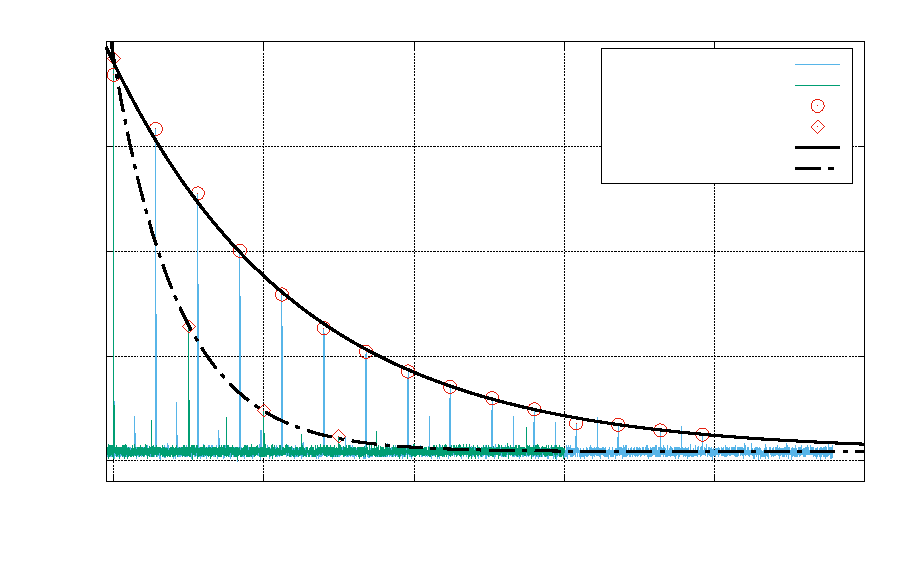
\includegraphics{waveform}}%
    \gplfronttext
  \end{picture}%
\endgroup

\caption{Representative waveform of pulse echo peaks, with the
  semi-automatically detected peaks marked, and single exponential
  decay mode fits for liquid water at two different pulse intervals,
  $\tau$. The noise background level has not been canceled in this
  plot, instead for this plot the fitted curves have been offsetted
  with said noise background. } 
\label{fig:waveform}
\end{figure*}

\begin{figure*}
\centering
% GNUPLOT: LaTeX picture with Postscript
\begingroup
  \makeatletter
  \providecommand\color[2][]{%
    \GenericError{(gnuplot) \space\space\space\@spaces}{%
      Package color not loaded in conjunction with
      terminal option `colourtext'%
    }{See the gnuplot documentation for explanation.%
    }{Either use 'blacktext' in gnuplot or load the package
      color.sty in LaTeX.}%
    \renewcommand\color[2][]{}%
  }%
  \providecommand\includegraphics[2][]{%
    \GenericError{(gnuplot) \space\space\space\@spaces}{%
      Package graphicx or graphics not loaded%
    }{See the gnuplot documentation for explanation.%
    }{The gnuplot epslatex terminal needs graphicx.sty or graphics.sty.}%
    \renewcommand\includegraphics[2][]{}%
  }%
  \providecommand\rotatebox[2]{#2}%
  \@ifundefined{ifGPcolor}{%
    \newif\ifGPcolor
    \GPcolortrue
  }{}%
  \@ifundefined{ifGPblacktext}{%
    \newif\ifGPblacktext
    \GPblacktexttrue
  }{}%
  % define a \g@addto@macro without @ in the name:
  \let\gplgaddtomacro\g@addto@macro
  % define empty templates for all commands taking text:
  \gdef\gplbacktext{}%
  \gdef\gplfronttext{}%
  \makeatother
  \ifGPblacktext
    % no textcolor at all
    \def\colorrgb#1{}%
    \def\colorgray#1{}%
  \else
    % gray or color?
    \ifGPcolor
      \def\colorrgb#1{\color[rgb]{#1}}%
      \def\colorgray#1{\color[gray]{#1}}%
      \expandafter\def\csname LTw\endcsname{\color{white}}%
      \expandafter\def\csname LTb\endcsname{\color{black}}%
      \expandafter\def\csname LTa\endcsname{\color{black}}%
      \expandafter\def\csname LT0\endcsname{\color[rgb]{1,0,0}}%
      \expandafter\def\csname LT1\endcsname{\color[rgb]{0,1,0}}%
      \expandafter\def\csname LT2\endcsname{\color[rgb]{0,0,1}}%
      \expandafter\def\csname LT3\endcsname{\color[rgb]{1,0,1}}%
      \expandafter\def\csname LT4\endcsname{\color[rgb]{0,1,1}}%
      \expandafter\def\csname LT5\endcsname{\color[rgb]{1,1,0}}%
      \expandafter\def\csname LT6\endcsname{\color[rgb]{0,0,0}}%
      \expandafter\def\csname LT7\endcsname{\color[rgb]{1,0.3,0}}%
      \expandafter\def\csname LT8\endcsname{\color[rgb]{0.5,0.5,0.5}}%
    \else
      % gray
      \def\colorrgb#1{\color{black}}%
      \def\colorgray#1{\color[gray]{#1}}%
      \expandafter\def\csname LTw\endcsname{\color{white}}%
      \expandafter\def\csname LTb\endcsname{\color{black}}%
      \expandafter\def\csname LTa\endcsname{\color{black}}%
      \expandafter\def\csname LT0\endcsname{\color{black}}%
      \expandafter\def\csname LT1\endcsname{\color{black}}%
      \expandafter\def\csname LT2\endcsname{\color{black}}%
      \expandafter\def\csname LT3\endcsname{\color{black}}%
      \expandafter\def\csname LT4\endcsname{\color{black}}%
      \expandafter\def\csname LT5\endcsname{\color{black}}%
      \expandafter\def\csname LT6\endcsname{\color{black}}%
      \expandafter\def\csname LT7\endcsname{\color{black}}%
      \expandafter\def\csname LT8\endcsname{\color{black}}%
    \fi
  \fi
    \setlength{\unitlength}{0.0500bp}%
    \ifx\gptboxheight\undefined%
      \newlength{\gptboxheight}%
      \newlength{\gptboxwidth}%
      \newsavebox{\gptboxtext}%
    \fi%
    \setlength{\fboxrule}{0.5pt}%
    \setlength{\fboxsep}{1pt}%
\begin{picture}(8502.00,5102.00)%
    \gplgaddtomacro\gplbacktext{%
      \csname LTb\endcsname%
      \put(860,1089){\makebox(0,0)[r]{\strut{}$10^-1$}}%
      \csname LTb\endcsname%
      \put(860,3988){\makebox(0,0)[r]{\strut{}$10^0$}}%
      \csname LTb\endcsname%
      \put(1136,440){\makebox(0,0){\strut{}$0$}}%
      \csname LTb\endcsname%
      \put(1914,440){\makebox(0,0){\strut{}$50$}}%
      \csname LTb\endcsname%
      \put(2692,440){\makebox(0,0){\strut{}$100$}}%
      \csname LTb\endcsname%
      \put(3471,440){\makebox(0,0){\strut{}$150$}}%
      \csname LTb\endcsname%
      \put(4249,440){\makebox(0,0){\strut{}$200$}}%
      \csname LTb\endcsname%
      \put(5028,440){\makebox(0,0){\strut{}$250$}}%
      \csname LTb\endcsname%
      \put(5806,440){\makebox(0,0){\strut{}$300$}}%
      \csname LTb\endcsname%
      \put(6584,440){\makebox(0,0){\strut{}$350$}}%
      \csname LTb\endcsname%
      \put(7363,440){\makebox(0,0){\strut{}$400$}}%
      \csname LTb\endcsname%
      \put(8141,440){\makebox(0,0){\strut{}$450$}}%
    }%
    \gplgaddtomacro\gplfronttext{%
      \csname LTb\endcsname%
      \put(160,2750){\rotatebox{-270}{\makebox(0,0){\strut{}Peaks /[V] (above noise background level)}}}%
      \put(4560,140){\makebox(0,0){\strut{}$t$ /[$\unit{ms}$]}}%
      \csname LTb\endcsname%
      \put(7238,1653){\makebox(0,0)[r]{\strut{}\footnotesize Peaks, ex. wet paper}}%
      \csname LTb\endcsname%
      \put(7238,1453){\makebox(0,0)[r]{\strut{}\footnotesize Dual mode fit}}%
      \csname LTb\endcsname%
      \put(7238,1253){\makebox(0,0)[r]{\strut{}\footnotesize Single mode fit}}%
      \csname LTb\endcsname%
      \put(7238,1053){\makebox(0,0)[r]{\strut{}\footnotesize Peaks, liquid water}}%
      \csname LTb\endcsname%
      \put(7238,853){\makebox(0,0)[r]{\strut{}\footnotesize Single mode fit }}%
    }%
    \gplbacktext
    \put(0,0){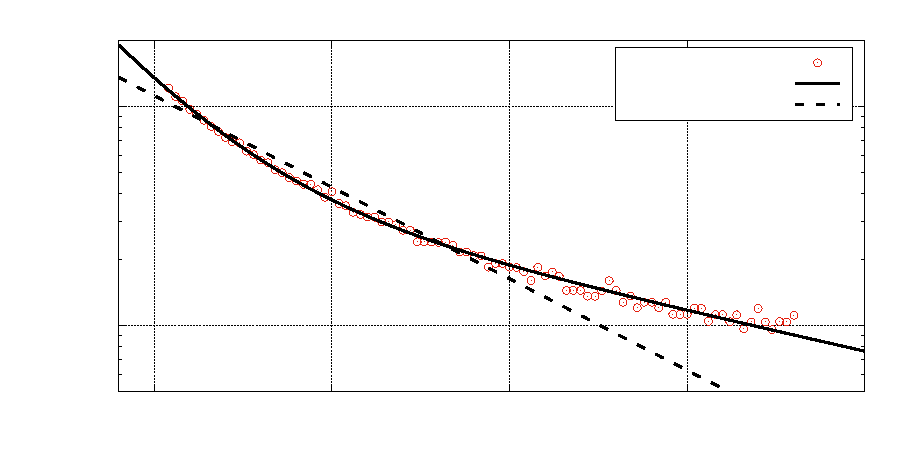
\includegraphics{peaks}}%
    \gplfronttext
  \end{picture}%
\endgroup

\caption{Detected pulse echo peaks from extra wet paper and liquid
  water together with single mode decay fits, and a dual mode decay
  fit for the extra wet paper. The liquid water peaks belong to the
  $\tau=\unit[28]{ms}$ measurement sown in \figref{fig:waveform}.
  The noise background level have been subtracted from the heights of
  the peaks. For a true single mode decay the peaks would thus all
  fall on a straight line in this log-plot, as shown by the liquid
  water peaks. } 
\label{fig:fitted-peaks}
\end{figure*}

As mentioned in the main report, the overall modus operandi is to
record the pulse echoes from the NMR apparatus on an oscilloscope, and
then from the saved waveform measure the decay rate of the pulse
echoes. This appendix aims to describe this process in a little more
detail. 

\figref{fig:waveform} shows two typical waveforms directly as they
were recorded from the oscilloscope. There were in general two
types of peaks in the waveform, the actual pulse echoes and then
sometimes the $\pi$ pulse generated unwanted glitches. These glitches
can be seen in the middle between two pulse echo peaks, e.g. in
\figref{fig:waveform} in the $\tau=\unit[28]{ms}$ waveform between
$t=\unit[500]{ms}$ and $t=\unit[800]{ms}$. A special script for
semi-automatic peak detection was therefore written and implemented. 
The ``semi-automatic'' part only means that the peaks were picked out
by the program, and then controlled visually by us to ensure that no
false peaks, like the $\pi$ pulse glitches, had been detected. 

The next thing to notice in \figref{fig:waveform} is that the
waveforms are all offsetted vertically by a small amount, which will
be called the noise background level (NBL). This NBL was estimated by
the \emph{median} of the oscilloscope signal after the last detected
peak. As a concrete example, the NBL for the $\tau=\unit[28]{ms}$
waveform in \figref{fig:waveform} is taken as the median of the
waveform after the peak at just below $t=\unit[800]{ms}$. 
The median was used for calculating the NBL since it is less sensitive
to rouge outliers in the data -- some of the recorded wave forms had
clear $\pi$ pulse glitches showing long after the last detected pulse
echo peak. Note that the NBL was individually calculated for each
waveform, althogh all our waveforms had an NBL of around 0.05\,V. 

Then the detected peaks, with the noise background level subtracted
from their heights, were fitted to either the single mode decay
\eqref{eq:multi-pulse_single} or the dual mode decay
\eqref{eq:multi-pulse_dual}, using Matlab's built-in \texttt{fit}
function~\cite{Matlab-fit}. This function also provided 95\,\%
confidence intervals for each fit parameter as well as
degree-of-freedom (DoF) adjusted coefficients of determination (R-squared
values). Supposedly this DoF adjustment is to
compensate for the number of fit parameters used. We do not know the
full details in either the confidence interval calculation or the DoF
adjustment, but we are confident in this built-in Matlab function. 



\subsection{Examples of single and dual mode decay}
The main report presents already calculated decay rates for a number
of different scenarios. It would be too much to show all the waveforms
and fits made for this work\footnotemark{}, but \figref{fig:waveform}
and~\ref{fig:fitted-peaks} present some representative examples. 
\footnotetext{Of course any raw-data, together with any related data
  anlysis, can be presented if requested. }

\figref{fig:waveform} shows two waveforms from the liquid water
diffusion measurement. The pulse echoe peaks and accompanying fits are
also shown. Notice that the $\tau=\unit[50]{ms}$ pule echoes are
decaying much faster than the $\tau=\unit[28]{ms}$ echoes. This is the
essence of the linear relationships, \eqref{eq:multi-pulse-rate},
shown in \figref{fig:water-pos}. 

Next \figref{fig:fitted-peaks} shows the difference between a single
mode and a dual mode decaying signal. In a log-plot, such as
\figref{fig:fitted-peaks}, the peaks from a single mode decay will lie
on a straight line, as is the case with the peaks from the liquid
water. We also clearly see that the peaks from extra wet paper
do not lie on a straigt line. They do however seem to follow a dual
mode decay well. This is the message conveyed by
\figref{fig:good-fit}, only that \figref{fig:good-fit} shows this same
message for every measured value. The extra wet paper peaks in
\figref{fig:fitted-peaks} are only an example, but it is a
representative example for all the measurements for both ``extra wet
printer paper'' and ``wet tissue paper''.



%%%%%%%%%%%%%%%%%%%%%%%%%%%%%%%%%%%%%%%%%%%%%%%%%%%%%%%%%%%%%%%%%%%%%%
\end{document}%% ^ ^ ^ ^ ^ ^ ^ ^ ^ ^ ^ ^ ^ ^ ^ ^ ^ ^ ^ ^ ^ ^ ^ ^ ^ ^ ^
%%%%%%%%%%%%%%%%%%%%%%%%%%%%%%%%%%%%%%%%%%%%%%%%%%%%%%%%%%%%%%%%%%%%%%



%  LocalWords:  Larmor coherentness diffusivity multi Batchelor DoF
%  LocalWords:  Matlab's Meiboom Matlab
